\newpage
\section{Bipolartransistoren}
	\begin{minipage}[c]{6cm}
		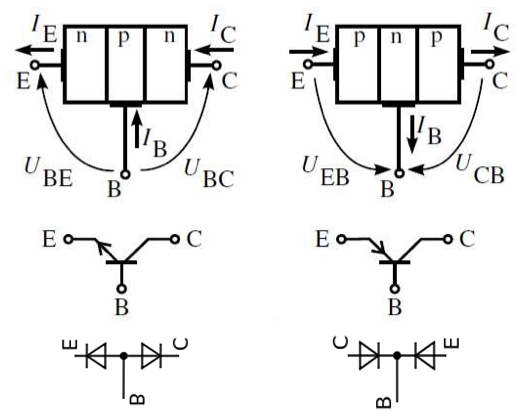
\includegraphics[width=5cm]{images/bipolarTransistor-Aufbau}
	\end{minipage}
	\begin{minipage}[c]{12cm}
		Links: NPN-Transistor \\
		Rechts: PNP-Transistor \\
		\\
		Die Schichten sind ungleich dick (Basis sehr dünn) und unterschiedlich dotiert.
		Sobald die BE-Diode Leitet, werden Elektronen vom Kollektor zur Basis gezogen und
		fliessen dann weiter zum Emitter. So steuert der Basisstrom $I_B$ den 
		Kollektorstrom $I_C$. \\
	\end{minipage} \\
	
	\begin{multicols}{2}
	\subsection{Betriebszustände}
		\begin{tabular}{l l}
			Normalbetrieb (Verstärker) & $V_{BE} > 0$, $V_{BC} < 0$\\
			Sättigung (Schalter EIN) & $V_{BE} > 0$, $V_{BC} > 0$\\
			Sperrbetrieb (Schalter AUS) & $V_{BE} < 0$, $V_{BC} < 0$\\
			Inversbetrieb (k. Anwendung) & $V_{BE} < 0$, $V_{BC} > 0$
		\end{tabular} \\
	\columnbreak
	\subsection{Stromverstärkungs-Faktoren}
		\begin{minipage}[c]{2.8cm}
			Basisschaltung \\
			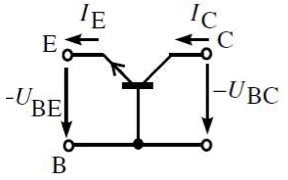
\includegraphics[width=2.8cm]{images/bip-basissch}\\
			$A_N=\frac{I_C}{I_E}$ \\
		\end{minipage}
		\begin{minipage}[c]{2.8cm}
			Emitterschaltung
			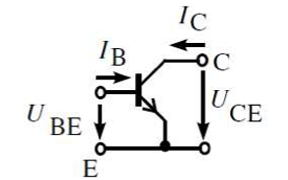
\includegraphics[width=2.8cm]{images/bip-emittersch}\\
			$B_N=\frac{I_C}{I_B}=\frac{A_N}{1-A_N}$ \\
		\end{minipage}
		\begin{minipage}[c]{2.8cm}
			Kollektorschaltung
			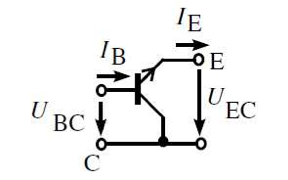
\includegraphics[width=2.8cm]{images/bip-kollektorsch}\\
			$C_N=\frac{I_E}{I_B}=\frac{1}{1-A_N}$ \\
		\end{minipage}
	\end{multicols}
	
	\subsection{Ebers-Moll-Modell}
		\begin{minipage}[c]{6cm}
			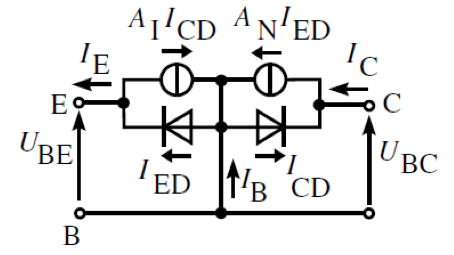
\includegraphics[width=5.2cm]{images/bipolar-EbersMoll}
		\end{minipage}
		\begin{minipage}[c]{8cm} 
			\begin{tabular}{l l}
			Kollektorstrom: & \fbox{$I_C=A_NI_{E_{sat}}\left(e^{\frac{U_{BE}}{U_T}}-1\right)
			 -I_{C_{sat}}\left(e^{\frac{U_{BC}}{U_T}}-1\right)$ }\\
			Emitterstrom: & \rule{0pt}{6ex}\fbox{$I_E=I_{E_{sat}}\left(e^{\frac{U_{BE}}{U_T}}-1\right)
			 -A_II_{C_{sat}}\left(e^{\frac{U_{BC}}{U_T}}-1\right)$} \\
			Basisstrom: & \rule{0pt}{4ex}\fbox{$I_B=I_E-I_C$} \\
			\end{tabular} 
		\end{minipage}
	
	\subsection{Kennlinien \& Formeln}
		\begin{minipage}[c]{12cm}
			{\bf Ausgangskennlinie (I)}\\
				typ.: $U_{CE_{sat}}=0.3V$ und Ausgangswiderstand $r_{CE} \approx \frac{U_{Early}}{I_{C0}}$\\
				\hspace{2mm}
			{\bf Stromübertragungskennlinie (II)}\\
				Kollektorstrom: $I_C = B_N \cdot I_B + I_{CE0} \approx B_N \cdot I_B$\\
				\hspace{2mm}	
			{\bf Eingangskennlinie (III)}\\
				Basisstrom: \smash{$I_B = I_{B_{sat}} \cdot (e^{\frac{U_{BE}}{U_T}}-1)$}\\
				Kleinsignalwiderstand: $r_{BE} = \frac{m\cdot U_T}{I_{B0}}$ mit $I_{B0}$: Arbeitspunktstrom\\
				\hspace{2mm}
			{\bf Spannungsrückwirkungskennlinie (IV)}\\
				$U_{BE} = \eta \cdot U_{CE}$ mit $\eta \approx 0.1 \%$ (kann meist vernachlässigt werden!)\\
        \end{minipage}	
		\begin{minipage}[c]{5cm}
			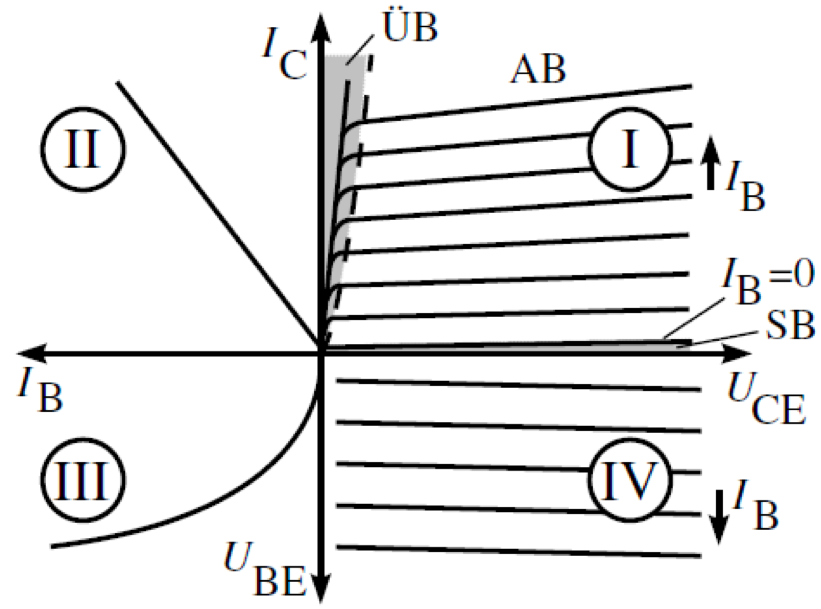
\includegraphics[width=5cm]{./images/BipTraKennlinien.png}
		\end{minipage}
		
	\subsection{Frequenzverhalten}
		\begin{minipage}{4cm}
			Kapazitäten: \\
			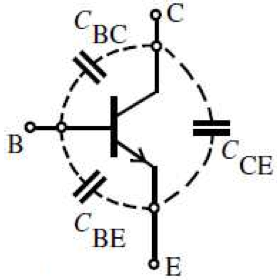
\includegraphics[width=3cm]{./images/bip-frequenz-cs}
		\end{minipage}	
		\begin{minipage}{6cm}
			Ersatzschaltbild: \\
			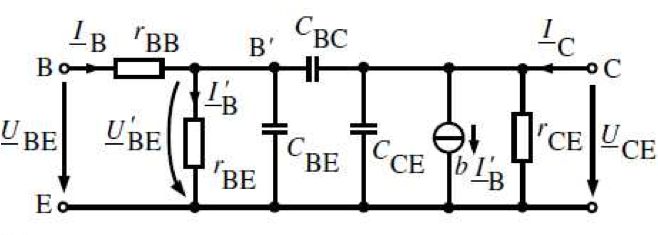
\includegraphics[width=6cm]{./images/bip-frequenz}
		\end{minipage}
		\begin{minipage}{6cm}
			\[ \underline{h}_{21e} (\omega) \approx \frac{b}{1 + r_{BE} \cdot \left(C_E + C_{BE} \right) \cdot j\omega} \] \\
			Bei der Transitfrequenz $\omega_t$ ist $h_{21e} = 1$.
		\end{minipage}
	
	\subsection{Early-Effekt}
		\begin{minipage}[c]{5cm}
			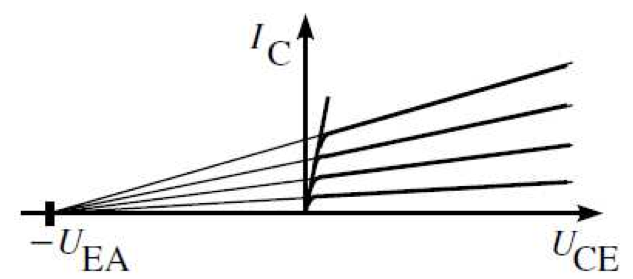
\includegraphics[width=5cm]{images/early-effekt}
		\end{minipage}
		\begin{minipage}[c]{12cm}
			Anstieg der Ausgangskennlinien beruht auf Veränderung der Basisweite infolge
			der Spannungsabhängigkeit der Sperrschichtweite der Basis-Kollektor-Diode. \\
			$U_{EA}$: Early-Spannung, Schnittpunkt der Ausgangskurven \\
			\\
			Modellerweiterung zur Berücksichtigung des Early-Effekts: \\
			$I_C = (B_NI_B+I_{CE_0})(1+\frac{U_{CE}}{U_{EA}})$
		\end{minipage}
				
	\subsection{Temperaturverhalten}
		Die maximale Leistung $P_V$ des Transistors muss stets kleiner als 
		$U_{CE} \cdot I_C$ sein. (Näherung)
		Zusätzlich muss die Wärme auch über das Gehäuse abgeführt werden können. Deshalb
		darf $P_V$ maximal $\frac{T_{max}-T_{amb}}{R_{th}}$ sein. ($R_{th}$: Thermischer
		Widerstand des Gehäuse) \\
		Der Transistor hat grundsätzlich das gleiche Temperaturverhalten wie die Diode. Somit
		gilt auch hier: $V_{BE}$ ändert um $-2\frac{mV}{K}$. Somit gilt für den
		Stromverstärkungsfaktor: $B_N=B_N(T_0)\cdot e^{C_b(T-T_0})$ mit 
		$C_b \approx 0.6\% \cdot K^{-1}$. \\
				
	\subsection{Kleinsignalverhalten}
		Beim Kleinsignal-Ersatzschaltbild wird das Verhalten des Transistors im Arbeitspunkt
		approximiert . Dazu wird ein Arbeitspunkt $AP$ im Kennlinienfeld eingezeichnet
		und dort linearisiert. \\
		\begin{minipage}[c]{6cm}
			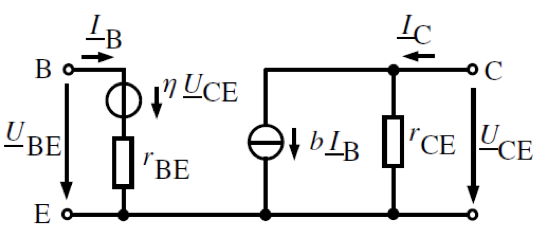
\includegraphics[width=6cm]{images/bip-kleinsignal}
		\end{minipage}
		\begin{minipage}[c]{6cm}
			$h_{11e} = r_{BE} = \frac{dU_{BE}}{dI_{B}} = \frac{m \cdot U_T}{I_{B_0}}$ \\
			$h_{12e} = \eta = \frac{dU_{BE}}{dU_{CE}} \approx 0$ \\
			$h_{21e} = b = \frac{dI_C}{dI_B} = B_N(1+\frac{U_{CE_0}}{U_{EA}}) \approx B_N$ \\
			$h_{22e} = \frac{1}{r_{CE}} = \frac{dI_C}{dU_{CE}} = \frac{I_{C0}}{U_{EA}}$ \\
			$S = \frac{b}{r_{BE}} = \frac{I_C}{m \cdot U_T}$
		\end{minipage}
		\begin{minipage}[c]{6cm}
			$r_{BE}$: Kleinsignal-Eingangswiderstand \\
			$\eta$: Kleinsignal-Spannungsrückwirkung \\
			$b$: Kleinsignal-Stromverstärkung \\
			$r_{CE}$: Kleinsignal-Ausgangswiderstand \\
			$S$: Kleinsignal-Steilheit
		\end{minipage} \\
		Kleinsignalmodell ohne Rückwirkung: $\eta \cdot U_{CE}$ wird weggelassen, weil 
		$\eta \approx 0$. Somit gilt: \\
		\begin{center}
			\fbox{$U_{BE} = r_{BE} \cdot I_B$} \hspace{1cm} und \hspace{1cm}
			\fbox{$I_C = b \cdot I_B + \frac{1}{r_{CE}} \cdot U_{CE}$} \hspace{1cm} und \hspace{1cm}
			\fbox{$b \cdot \underline{I}_B = S \cdot \underline{U}_{BE}$}
		\end{center}
		
		Somit gilt für die \textbf{Emitterschaltung}: \\
		\begin{minipage}[c]{6cm}
			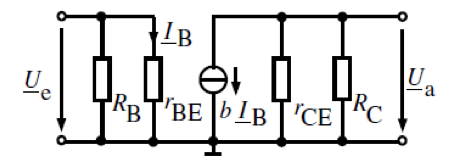
\includegraphics[width=6cm]{images/emittersch-esb}
		\end{minipage}
		\begin{minipage}[c]{12cm}
			$U_a = -b \cdot I_B \cdot (R_C || r_{CE})$ und $I_B=\frac{U_e}{r_{BE}}$ \\
			somit: $V_u = \frac{U_a}{U_e} = -\frac{b(R_C || r_{CE})}{r_{BE}}$ 
		\end{minipage} \\
		
	\subsection{Transistor als Schalter}
		\begin{minipage}[c]{12cm}
			Der Transistorschalter besitzt zwei stationäre Arbeitspunkte: \\
			
			\textbf{AP1:} Arbeitspunkt EIN, hoher Stromfluss, Transistor übersteuert. \\
			Sättigungsspannung: $U_{CE_{sat}} \approx 100mV$ \\
			Übersteuerungsgrad: $m = \frac{B_N \cdot I_{B_1}}{I_{C_1}}$ mit
			$I_{B_1}=\frac{U_{E_1}-U_{BE_1}}{R_B}$ und $U_{C_1}=\frac{U_{0_C}-U_{CE_1}}{R_C}$ \\
			
			\textbf{AP2:} Arbeitspunkt AUS, kein Stromfluss, Transistor gesperrt. \\
			$I_B = 0$, $I_C = 0$, $U_{out} = U_{0_C}$
		\end{minipage}
		\begin{minipage}[c]{5cm}
			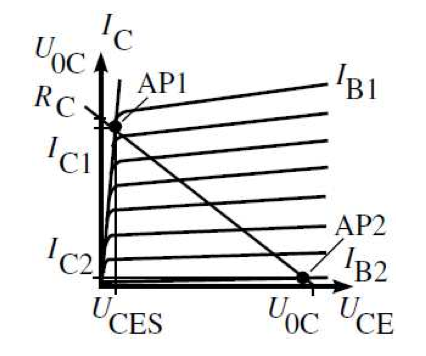
\includegraphics[width=5cm]{images/bip-schalter-ap}
		\end{minipage} \\
		
		\subsubsection{Dynamisches Verhalten}
		Das zeitliche Verhalten bei Schaltvorgängen wird in erster Linie durch die
		Transistorkapazitäten bestimmt. Beim Einschaltvorgang tritt zuerst eine
		Einschaltverzögerung $t_d$ auf (bis $I_C$ überhaupt reagiert), dann dauert es
		eine Anstiegszeit $t_a$ bis der Strom $I_C$ erreicht ist. Beim Ausschaltvorgang
		passiert eine Speicherzeit $t_s$ lang nichts, dann braucht es eine Abfallzeit $t_f$
		bis der Strom $I_C=0$ wird.  \\
		Zur Reduktion der Speicherzeit $t_s$ kann eine Schottkydiode von der Basis zum 
		Kollektor geschalten werden. Somit wird $U_{BC}$ limitiert und die Ladung verkleinert.
		Diese Methode wurde in der 74S- und der 74LS-Familie eingesetzt. \\

        \subsubsection{Gegenkopplung}

            \begin{minipage}{5.5cm}
                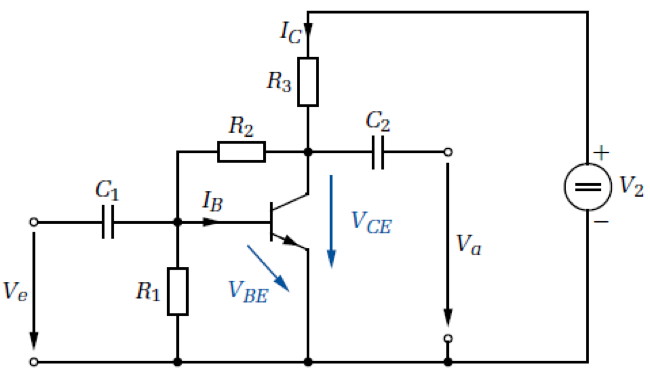
\includegraphics[height=2.5cm]{./images/Spannungsgegenkopplung.png} \\
                Gegenkopplung durch $R_2$
            \end{minipage}
            \begin{minipage}{5.5cm}
                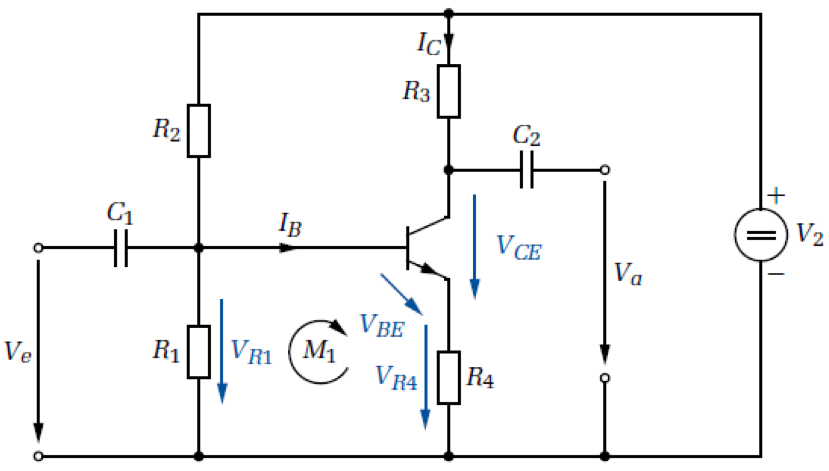
\includegraphics[height=2.5cm]{./images/Stromgegenkopplung.png} \\
                Gegenkopplung durch $R_4$\\
                $V_{out} = -\frac{R_3}{R_4}\cdot V_{in}$\\
            \end{minipage} 
            \begin{minipage}{5.5cm}
         	Motivation: Durch Gegenkopplung wird die Verstärkung des Transistors kleiner, doch
         	Bauteiltoleranzen, Temperaturschwankungen und Verzerrungen werden minimiert.                
            \end{minipage}
            
        \subsubsection{Transistorverstärkerschaltungen}
            \begin{minipage}[T]{4.7cm}
                Emitterschaltung mit\\
                Stromgegenkopplung\\
                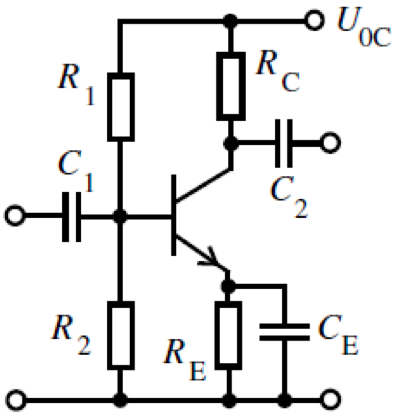
\includegraphics[height=3cm]{./images/BipTraEmitterschStGk.png}
            \end{minipage}
            \begin{minipage}[T]{4.7cm}
                Emitterschaltung mit\\
                Spannungsgegenkopplung\\
                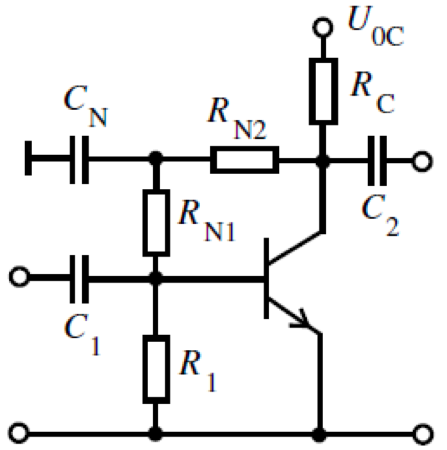
\includegraphics[height=3cm]{./images/BipTraEmitterschSpGk.png}
            \end{minipage}
            \begin{minipage}[T]{5.7cm}
                Basisschaltung\\\\
                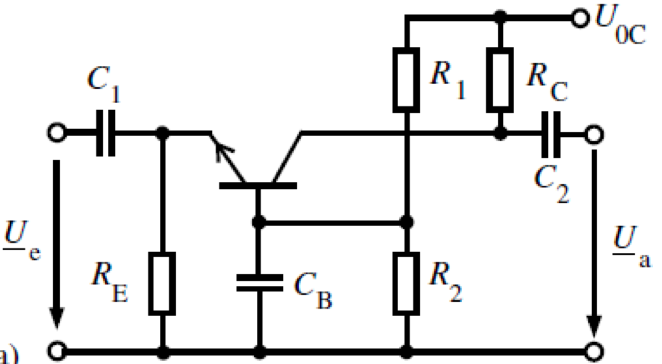
\includegraphics[height=3cm]{./images/BipTraBasissch.png}
            \end{minipage}
            \begin{minipage}[T]{3.7cm}
                Kollektorschaltung\\\\
                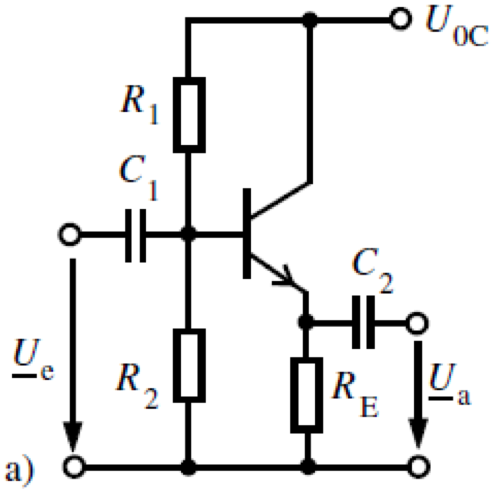
\includegraphics[height=3cm]{./images/BipTraKollektorsch.png}
            \end{minipage}

		\begin{multicols}{2}
		\subsubsection{Stromspiegel}
			\begin{minipage}{3.5cm}
				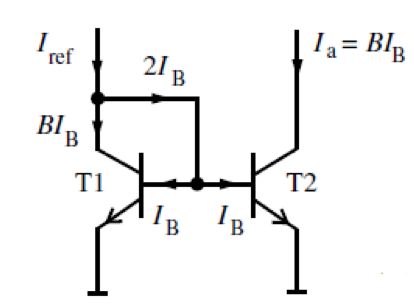
\includegraphics[width=3.5cm]{./images/stromspiegel}
			\end{minipage}
			\begin{minipage}{4.5cm}
				\begin{equation*}
					I_a \approx I_{ref} \textbf{, da } B \gg 1 \textbf{ und } I_B \ll I_{ref}
				\end{equation*}
			\end{minipage}

		\subsubsection{Widlar-Stromspiegel}
			\begin{minipage}{4cm}
				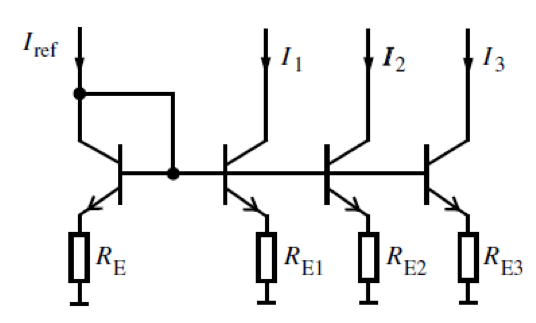
\includegraphics[width=4cm]{./images/stromspiegel-widlar}
			\end{minipage}
			\begin{minipage}{4cm}
				Ströme $I_1 \dots I_3$ werden einzeln durch Widerstandsverhältnisse gewichtet: \\
				\begin{equation*}
					I_1 = I_{ref} \cdot \frac{R_E}{R_{E1}}
				\end{equation*}
			\end{minipage}	

		\subsubsection{Stromspiegel mit Kaskode}
			\begin{minipage}{3.5cm}
				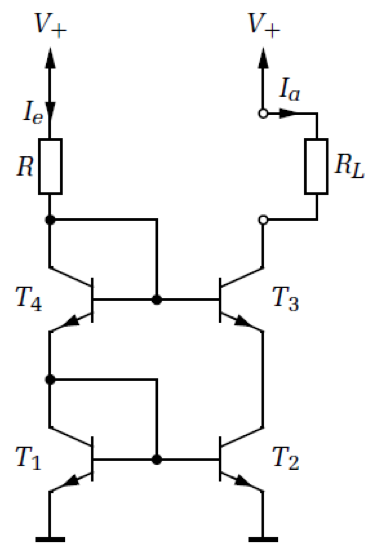
\includegraphics[width=3.5cm]{./images/stromspiegel-kaskode} 
			\end{minipage}
			\begin{minipage}{4.5cm}
				$T_1$ als Diode geschaltet, bestimmt $V_{BE2}$ und damit $I_C$ von $T_2,T_3$ \\\\
				$T_4$ als Diode geschaltet, bestimmt $V_{BE3}$ und damit den Arbeitspunkt \\\\
				$T_3$ in Basisschaltung, tiefer Eingangswiderstand, kaum Änderung von $U_{C2}$ und damit kaum Stromänderung
			\end{minipage}
		\end{multicols}
							
         \subsubsection{Differenzverstärker}
             \begin{minipage}[T]{12cm}
             	Der Differenzverstärker ist symmetrisch, d.h. $U_{a1} - U_{a_{AP}} = U_{a_{AP}} - U_{a2}$ \\
             	
             	\begin{tabular}{ll}
             	differentieller Eingangswiderstand & $r_e = 2 \cdot r_{BE}$ \\
             	differentieller Ausgangswiderstand & $r_a = (R_C || r_{CE})$ \\
				Differenz-Verstärkung & $v_d = \frac{U_{A_d}}{U_{E_d}} = -S\cdot r_A \approx -S\cdot R_C$ \\
				Gleichtaktverstärkung &  $v_{gl} = -\frac{R_C}{2\cdot R_E}$ \\
				Gleichtaktunterdrückung & $G = \frac{v_d}{v_{gl}} = 2\cdot S \cdot R_E$
				\end{tabular}
             \end{minipage}
             \begin{minipage}{4cm}
                 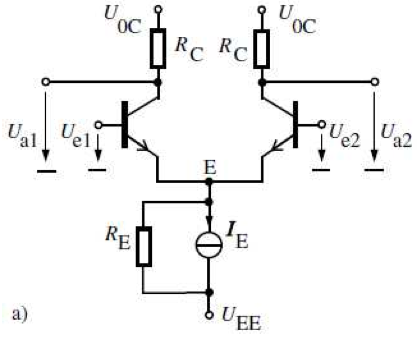
\includegraphics[height=4cm]{./images/BipTraDiffAmp.png}
             \end{minipage}\\
             
         \subsubsection{Leistungsendstufen}
             \begin{minipage}[T]{4.7cm}
                 Klasse A-Verstärker \\
                 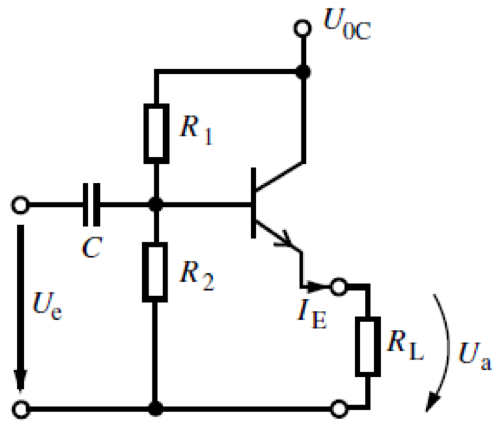
\includegraphics[height=4cm]{./images/KlassA_Amp.png} \\
                 	$ \eta = \frac{P_\sim}{P_=} \leq 25 \% $
             \end{minipage}
             \begin{minipage}[T]{4.7cm}
                 Klasse B-Verstärker \\
                 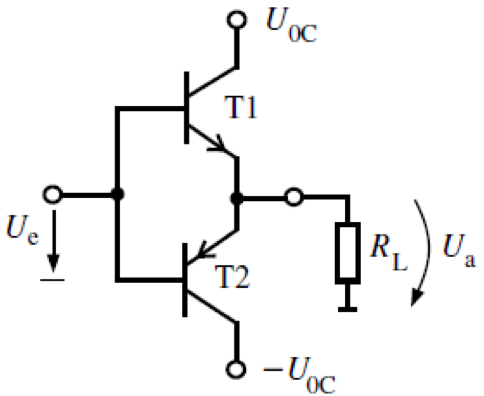
\includegraphics[height=4cm]{./images/KlassB_Amp.png} \\
                 	$ \eta \leq 78,5 \% $
             \end{minipage}
             \begin{minipage}[T]{4.7cm}
                 Klasse AB-Verstärker\\
                 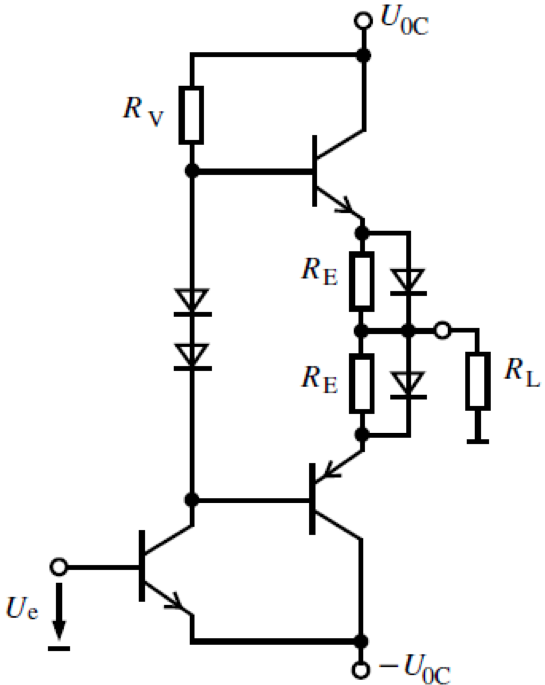
\includegraphics[height=4cm]{./images/KlassAB_Amp.png}
             \end{minipage}
             \begin{minipage}[T]{4.7cm}
                 Arbeitspunkte jeweiler Klassen\\\\
                 \vspace{5mm}
                 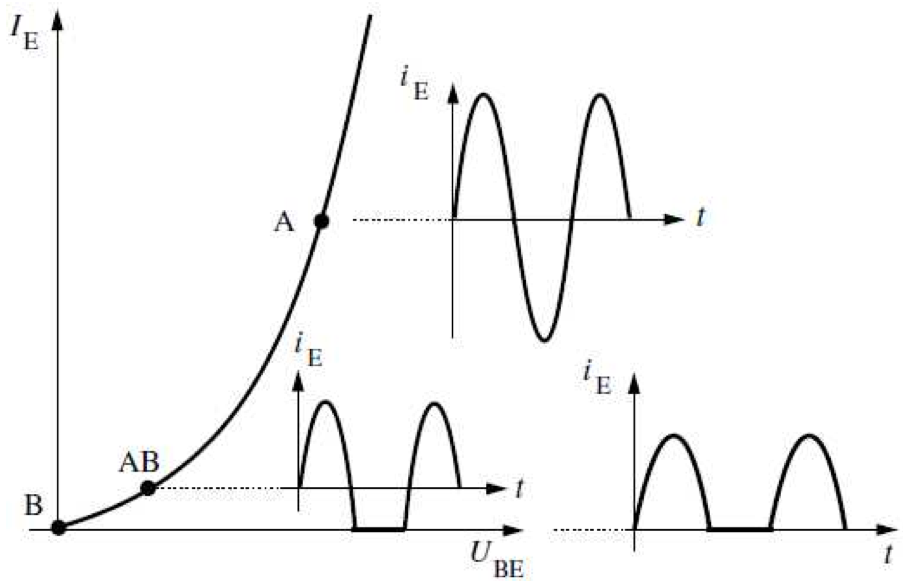
\includegraphics[width=4.7cm]{./images/EndstufenAP.png}
             \end{minipage}		